\documentclass{article}
\usepackage{graphicx} % Required for inserting images
\usepackage{float}
\title{Miscelanea 2da unidad}
\author{Carlos Flores}
\date{April 2024}

\begin{document}

\maketitle

\section{Introduction}

\subsection*{Punto fijo para sistemas no lineales }
\begin{enumerate}
    \item $x^2 + y^2 = 10$ \\
    $xy + y^3 = 7$ \\
    $(x, y) = (1.5, 1.5)$       
    
    \item $2x_1 - x_2 - e^{-x_1} = 0$ \\
    $-x_1 + 2x_2 - e^{-x_2} = 0$
\end{enumerate}

\subsection*{Método de Newton }
\begin{enumerate}
    \item $x^3 - 3xy^3 = 1$ \\
    $3x^3y - y^3 = 0$
    
    \item $3x_1 - \cos(x_2x_3) - \frac{1}{2} = 0$ \\
    $x_2^2 - 81(x_2 + 0.1)^2 + \sin(x_3) + 1.06 = 0$ \\
    $e^{-x_1x_2} + 20x_3 + 10\pi - \frac{3}{3} = 0$
\end{enumerate}


{En  los dos primeros sistemas resuelvo hasta el punto 3 donde sacamos las derivadas parciales a mano, subo las imágenes de lo aplicado y me refuerzo con el código
las derivadas van a ir en la función convergencia y el formato iterativo va a ir en la función g_1, g_2 respectivamente

El tercer sistema del el código está súper complejo por el echo de meter el jacobiano no sé si lo tenga listo para la entrega me está costando demaciado . Y del 4to sistema el código veo imposible su entrega pero trataré de avanzar lo más que se pueda}
\section{primer sistema}

\begin{figure}
            \centering
            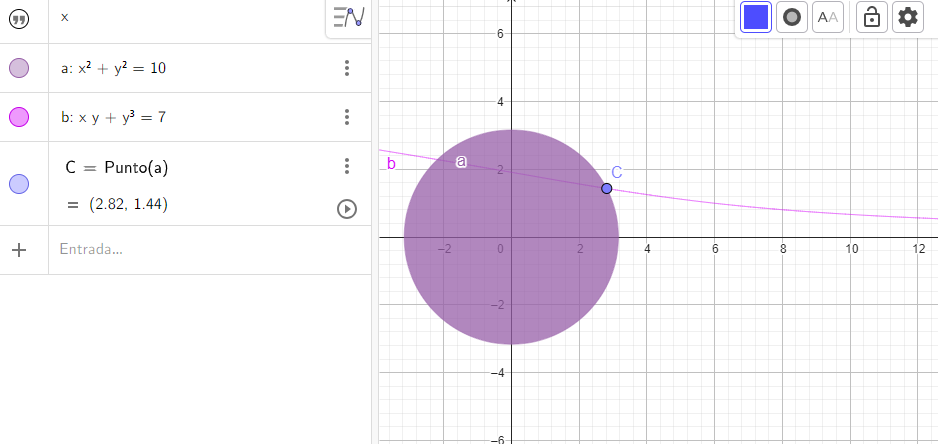
\includegraphics[width=1.5\linewidth]{puntio fijo para el primer sistema.PNG}
            \caption{primer sistema graficado en geogebra}
            \label{fig:enter-label}
        \end{figure}
        
\item en este sistema tomamos en cuenta las funciones en geogebra y nos da el resultado de la imagen 


\begin{figure}
            \centering
            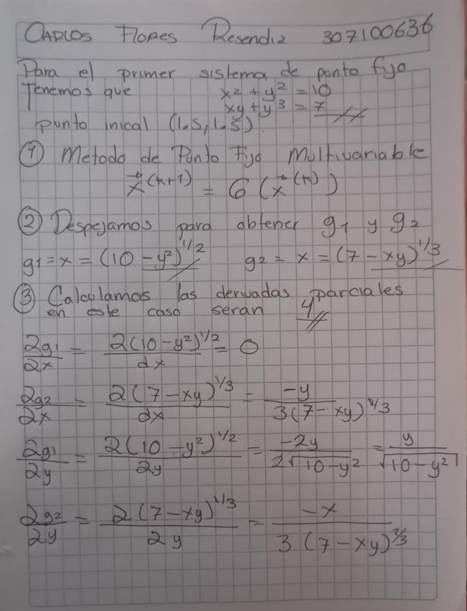
\includegraphics[width=1\linewidth]{derivadas parciales 1er sistema.PNG}
            \caption{Aqui termino el primer sistema ya que en el codigo ago las iteraciones y el calculo del error aqui dejo las derivas parciales en imagen}
            \label{blackhole}
    
\end{figure}


\begin{figure}
        \centering
        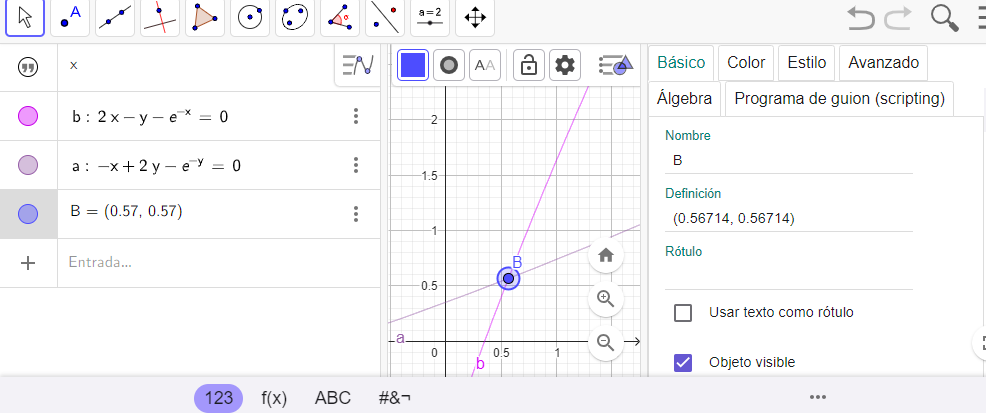
\includegraphics[width=1.5\linewidth]{punto fijo 2do sistema.PNG}
        \caption{geogebra segundo sistema de ecuaciones del método de punto fijo }
        \label{fig:enter-label}
    \end{figure}


\begin{figure}
        \centering
        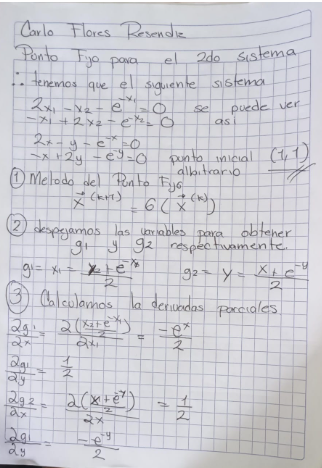
\includegraphics[width=1\linewidth]{derivadas parciales 2do sistema.PNG}
        \caption{En esta imagen calculamos las derivadas parciales de igual manera que el primer sistema de punto fijo llegamos a la solucion por medio del programa  }
        \label{fig:enter-label}
    \end{figure}


\begin{figure}
        \centering
        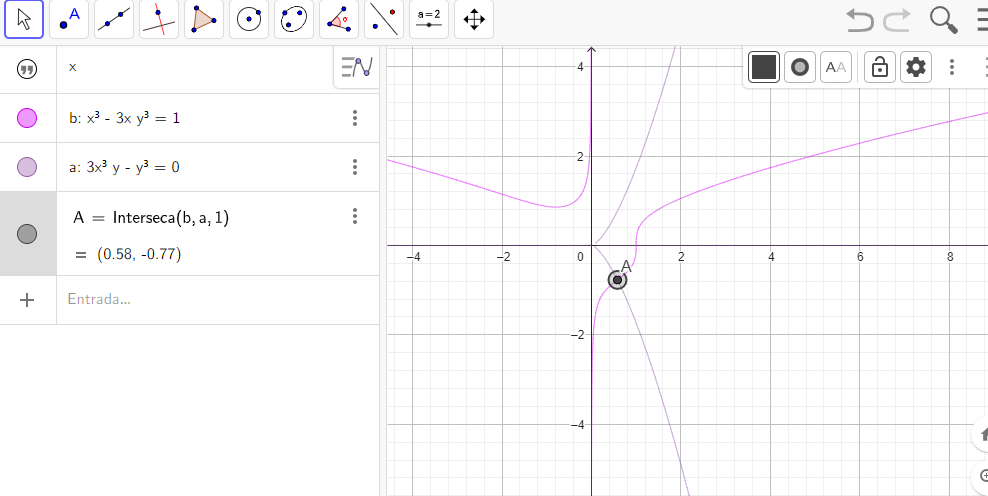
\includegraphics[width=1.5\linewidth]{raiz newton 3er sistema.PNG}
        \caption{En esta imagen podemos observar la solucion al sistema de newton la raiz}
        \label{fig:enter-label}
    \end{figure}
    
\begin{figure}
            \centering
            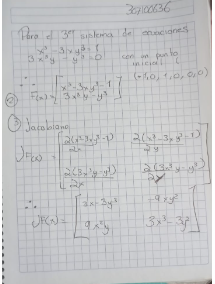
\includegraphics[width=.75\linewidth]{jacobiano del tercer sistema.PNG}
            \caption{en esta imagen se puede observar el jacobiano y basicamente  isetodo lo popsiblke porque el programa me diera resultados pero creo que falle }
            \label{fig:enter-label}
        \end{figure}
              
  
       





\end{document}
